%\documentclass{beamer} 
\documentclass[handout]{beamer} 
\usetheme{Ilmenau}
\usepackage{graphicx,verbatim,hyperref}
\usepackage{textpos}

\usecolortheme{beaver}
\useinnertheme{default}
\setbeamertemplate{itemize item}[triangle]
\setbeamertemplate{itemize subitem}[triangle]
\setbeamertemplate{itemize subsubitem}[circle]
\setbeamertemplate{enumerate items}[default]
\setbeamertemplate{blocks}[upper=block head,rounded]
\setbeamercolor{item}{fg=black}
\usefonttheme{serif} %should allow ccfonts to take effect

\usepackage{cite}
\usepackage{times, verbatim,xcolor,bm}
%\usepackage[usenames,dvipsnames]{color}
\usepackage{amsbsy,amssymb, amsmath, amsthm}
\usepackage{booktabs}
%David miller's fonts
	\usepackage[T1]{fontenc}
	\usepackage[boldsans]{ccfonts}
	%\usepackage[boldsans]{concmath}
	\usepackage[euler-hat-accent]{eulervm}

\newcommand{\al}{\alpha}
\newcommand{\expect}{\mathbb{E}}
\newcommand{\Bt}{B(\bm{\tau^a})}
\newcommand{\bta}{\bm{\tau^a}}
\newcommand{\btn}{\bm{\tau^{tw}}}
\newcommand{\ga}{\gamma}
\newcommand{\ve}{\varepsilon}
\newcommand{\ta}{\theta}
\newcommand{\de}{\delta}
\newcommand{\ov}{\overline}
\newcommand{\un}{\underline}

\newenvironment{changemargin}[2]{% 
  \begin{list}{}{% 
    \setlength{\topsep}{0pt}% 
    \setlength{\leftmargin}{#1}% 
    \setlength{\rightmargin}{#2}% 
    \setlength{\listparindent}{\parindent}% 
    \setlength{\itemindent}{\parindent}% 
    \setlength{\parsep}{\parskip}% 
  }% 
  \item[]}{\end{list}} 
	
	\let\Tiny=\tiny


\title[Lobbying and Legislative Uncertainty\hspace{2.95in}\insertframenumber/\inserttotalframenumber]{Lobbying and Legislative Uncertainty}
%\author[Kristy Buzard]{Kristy Buzard \\ Syracuse University and The Wallis Institute \\ kbuzard@syr.edu}
\author[Kristy Buzard]{\texorpdfstring{Kristy Buzard\newline Syracuse University and The Wallis Institute  \newline\url{kbuzard@syr.edu}}{Kristy Buzard}}
\date{April 16, 2016}
\begin{document}
\maketitle
%\insertpresentationendpage removed b/c of appendix




\section{Overview}
\subsection{Overview}
\begin{frame}{The Questions}

\pause
\begin{enumerate}[<+->]
\item How does uncertainty about legislators' preferences impact 
	\begin{itemize}
		\item lobbying strategies (e.g. who to lobby, how much to `pay')
		\item probability a bill passes
	\end{itemize}
	\vskip.1in
\item Can we distentangle fundamental uncertainty about preferences from equilibrium and modeling uncertainty?
	\begin{itemize}
		\item[$\Rightarrow$] Build a structural model to take to U.S. House data
	\end{itemize}
	\vskip.1in
\item Ultimately, want to identify cross-industry measures of legislative uncertainty
\end{enumerate}

\end{frame}


\begin{frame}{Some Stylized Facts}

\pause
\begin{enumerate}[<+->]
	\item In the U.S., about $\$ 4$ billion / yr spent on lobbying and campaign contributions
	\item There is usually lobbying on both sides of a given issue
	\item Moderate legislators receive more contributions than those that are ideologically extreme
	\item Legislators about whom there is a moderate level of uncertainty are lobbied the most
\end{enumerate}

\pause
\vskip.2in
Adding uncertainty to standard model captures (2) --- (4)
\end{frame}

\begin{frame}{Literature}
\pause
\begin{itemize}[<+->]
	\item \textbf{Vote Buying in Legislatures}: Groseclose $\&$ Snyder 1996, Banks 2000, Dal Bo 2007
	\item \textbf{Lobbying with Uncertainty}: Coates $\&$ Ludema 2001, Le Breton $\&$ Salanie 2003, Le Breton $\&$ Zaphorozhets (2007)
	\item \textbf{Probabilistic Voting with Policy Motivation}: Roemer 1994, 1997, Duggan $\&$ Fey 2011
	%\item \textbf{Uncertainty}: 
\end{itemize}
\end{frame} 



%\begin{frame}
%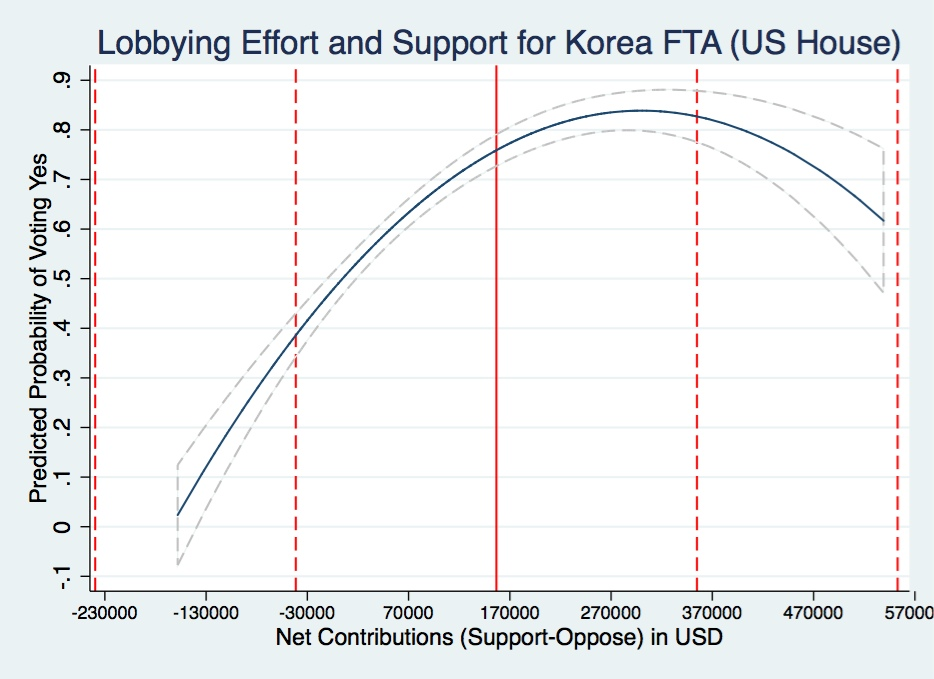
\includegraphics[height=2.75in, width=4.25in]{graph2.jpg}
%\end{frame}


\begin{frame}
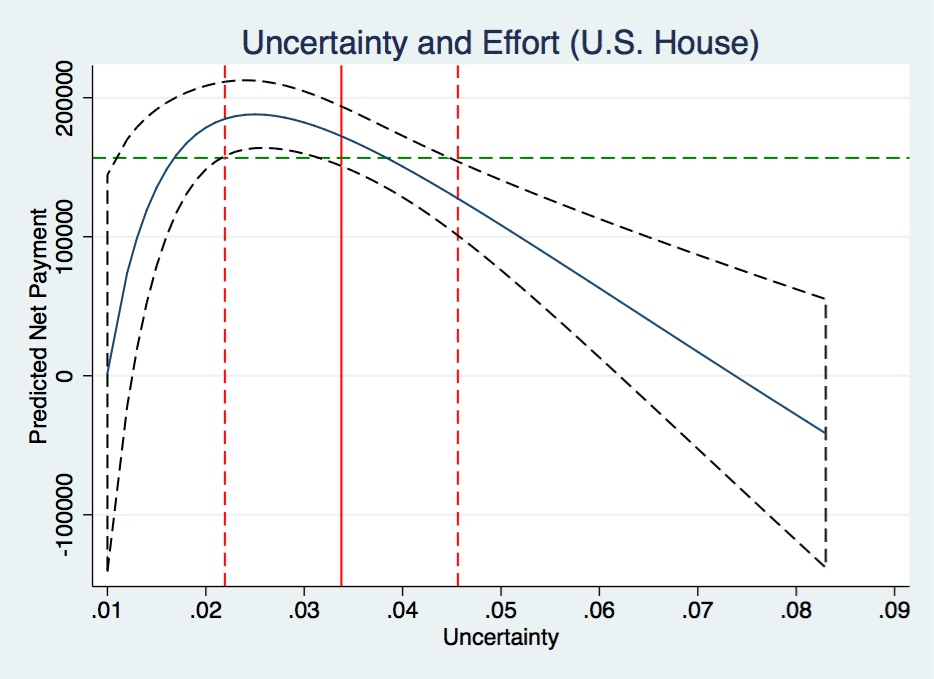
\includegraphics[height=2.75in, width=4.25in]{graph1.jpg}
\end{frame}


\begin{frame}{Preview}
\frametitle{Context}
\pause
U.S. House of Representative 
\pause
\begin{itemize}[<+->]
	\item All roll call votes, 2005 through present
	\item Interest group lobbying on each vote
	\item PAC contributions, LDA lobbying data
\end{itemize}

\vskip.2in
\pause
Use multi-dimensional ideal-point estimation to identify measures of uncertainty
\end{frame}

\begin{frame}
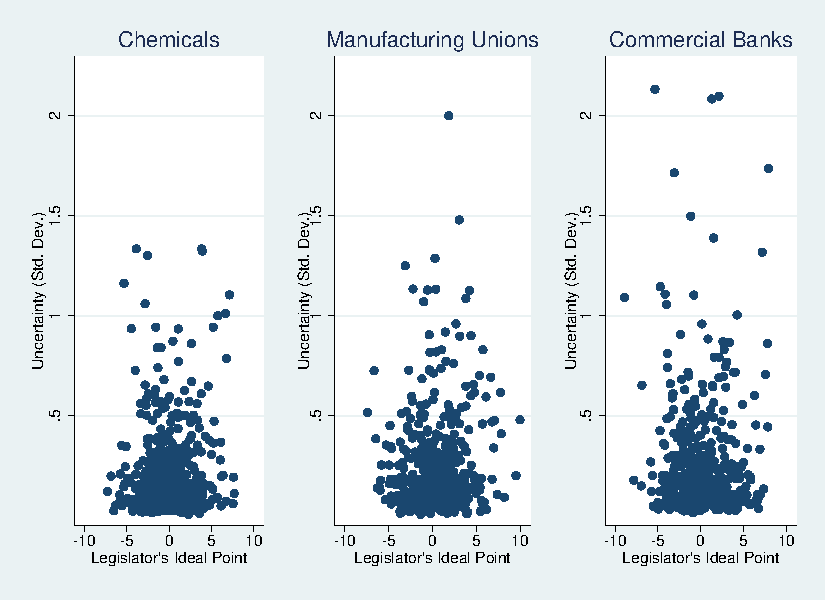
\includegraphics[height=2.75in, width=4.25in]{NSF_combined_graph.pdf}
\end{frame}





\section{Model}
\subsection{Political Structure}
\begin{frame}{Policy and Politics}

\pause
Three legislators
\pause
\begin{itemize}
	\item Identified by location in linear preference space: $i \in \left\{-0.5,0,.5\right\}$
	\item Each will vote for status quo $\bm{s}$ or new proposal $\bm{x}$
	\item Decision made by majority vote
\end{itemize}

\pause
\vskip.2in
Two vote buyers, $A$ and $B$
\pause
\begin{itemize}
	\item A prefers $x$, $B$ prefers $s$
\end{itemize}

\end{frame}



\begin{frame}{Timeline}
\pause
\begin{enumerate}[<+->]
	\item {\bfseries Vote Buyer A}
		\begin{enumerate}[i.]
			%\pause
			\item Chooses bribes $\un{a} = \left(a_{-.5},a_0,a_{.5}\right)$
		\end{enumerate}
	%\pause
	\item \textbf{Vote Buyer B}
		\begin{enumerate}[i.]
			%\pause
			\item Observes $\un{a}$
			%\pause
			\item Chooses bribes $\un{b} = \left(b_{-.5},b_0,b_{.5}\right)$
		\end{enumerate}
	%\pause
	\item \textbf{Legislature}
	%\pause
		\begin{enumerate}[i.]
			\item All legislators observe $\un{a},\un{b}$
			\item Uncertainty about preferences realized: $\un{\ta} = \left(\ta_{-.5},\ta_0,\ta_{.5}\right)$
			\item Each legislator votes for her preferred policy 
		\end{enumerate}
\end{enumerate}
\end{frame}


\subsection{The Players}

\begin{frame}{D}
\pause
  Objective function:
\pause
\[
  W = \mathit{CS}_X(\tau) + \ga(s,e) \pi_X(\tau) + \mathit{CS}_Y(\tau^*) + \pi_Y(\tau^*) + \mathit{TR}(\tau)
\]
\vskip-.1in
\pause
\begin{itemize}[<+->]
	\item S
		\begin{itemize}
			\item $s$: 
			\item $e$: 
		\end{itemize}
	\item Optimal 
		\begin{itemize}
			\item Ignores 
			\item Takes 
		\end{itemize}
\end{itemize}
\end{frame}


\begin{frame}{D}
\pause
  Objective function:
\pause
\[
  W = \mathit{CS}_X(\tau) + \ga(s,e) \pi_X(\tau) + \mathit{CS}_Y(\tau^*) + \pi_Y(\tau^*) + \mathit{TR}(\tau)
\]
\vskip-.1in
\pause
\begin{itemize}[<+->]
	\item S
		\begin{itemize}
			\item $s$: 
			\item $e$: 
		\end{itemize}
	\item Optimal 
		\begin{itemize}
			\item Ignores 
			\item Takes 
		\end{itemize}
\end{itemize}
\end{frame}


\begin{frame}
\frametitle{Political Pressure}
Two potential sources
\pause
\begin{enumerate}[<+->]
	\item Endogenous effort choice of lobby, $e$
		\begin{itemize}[<+->]
			\item Lobby chooses effort to maximize profits, $\pi(\cdot)$, net of lobbying effort, $e$
			\item Call lobby's optimal effort choice $e^L$
						\[
						  e^L = \max_e \pi(\tau(\ga(e))) - e
						\]
		\end{itemize}
\end{enumerate}

\end{frame}




\section{Results}
\subsection{One Vote Buyer}
\begin{frame}{}

\pause
When :

\pause
\begin{itemize}[<+->]
	\item T
	\item I
	\item C
\end{itemize}

\pause
\vskip.2in
\begin{beamerboxesrounded}[upper=palette tertiary, shadow=true]{Result...}
    When Vote Buyer $B$ pays bribes to exactly two legislators, the bribes are such that the two bribed legislators' ideal points gross of bribes are equalized. Which two legislators are bribed depends on the bias parameter $\al$.
\end{beamerboxesrounded}

\end{frame}


\begin{frame}{When ...}
Now 
\pause
\begin{itemize}[<+->]
	\item Want 
	\item But 
\end{itemize}

\pause
\vskip.2in
\begin{beamerboxesrounded}[upper=palette tertiary, shadow=true]{Result...}
    When Vote Buyer $B$ pays bribes to all three legislators, the bribes are such that the legislators' ideal points gross of bribes are equalized.
\end{beamerboxesrounded}
\end{frame}

\begin{frame}
\begin{beamerboxesrounded}[upper=palette tertiary, shadow=true]{Result...}
      When Vote Buyer $B$ pays bribes to exactly one legislator, it may be any one of the three legislators depending on the bias parameter $\al$.
\end{beamerboxesrounded}

\pause
\vskip.2in
\begin{beamerboxesrounded}[upper=palette tertiary, shadow=true]{Result...}
  When Vote Buyer $B$ has a low willingness to pay, he does not bribe any legislator.
\end{beamerboxesrounded}

\end{frame}


\begin{frame}{Varying Uncertainty Across Legislators}
Now 
\pause
\begin{itemize}[<+->]
	\item Want 
	\item But 
\end{itemize}

\pause
\vskip.2in
\begin{beamerboxesrounded}[upper=palette tertiary, shadow=true]{Conjecture}
 When there is no bias in the positions of the legislators ($\al =0$), the bribes of legislators whose ideal points are at the median in terms of uncertainty receive the highest relative bribes.\end{beamerboxesrounded}
\end{frame}

\subsection{Two Vote Buyers}
\begin{frame}
\begin{beamerboxesrounded}[upper=palette tertiary, shadow=true]{Result...}
  It is possible that neither vote buyer bribes any legislator on a given vote. This occurs when both vote buyers' willingness-to-pay parameters are small.
\end{beamerboxesrounded}

\pause
\vskip.2in
\begin{beamerboxesrounded}[upper=palette tertiary, shadow=true]{Result...}
  It is possible for both vote buyers to bribe legislators on the same vote.
\end{beamerboxesrounded}

\end{frame}



\section{Conclusion}

\begin{frame}{Future Work}
\pause
\begin{itemize}[<+->]
	\item A
	\item I
	\item C
\end{itemize}

\end{frame}


\begin{frame}{Conclusion}
Taking into account
\pause
\begin{itemize}[<+->]
		\item provides 
		\item demonstrates 
		\item helps 
\end{itemize}

\end{frame}


\end{document}